\documentclass[9pt,twocolumn,twoside]{rilabRxiv}
% Use the documentclass option 'lineno' to view line numbers
\usepackage{blindtext}
\usepackage{hyperref}

\usepackage[textsize=tiny,colorinlistoftodos]{todonotes} % comments in margins
\setlength{\marginparwidth}{1cm}
\definecolor{cornflowerblue}{rgb}{0.39, 0.58, 0.93}

%%%%%%%Add comments in color
\newcommand{\ms}[1]{{\small \textcolor{green}{#1}}}
\newcommand{\jri}[1]{{\small \textcolor{red}{#1}}}
\newcommand{\citex}[1]{{\small \textcolor{red}{CITE(#1)}}}
\newcommand{\X}{{\textcolor{red}{X}}}

\newcolumntype{b}{X}
\newcolumntype{s}{>{\hsize=.5\hsize}X}

% Set supplement numbers to S and start counting newly
\newcommand{\beginsupplement}{%
        \setcounter{table}{0}
        \renewcommand{\thetable}{S\arabic{table}}%
        \setcounter{figure}{0}
        \renewcommand{\thefigure}{S\arabic{figure}}%
     }


\title{Maize domestication and gene interaction}

\author[$\ast$,1]{Michelle C Stitzer}
\author[$\ast,\dagger$]{Jeffrey Ross-Ibarra}
%\author[$\ast$,$\ddagger$,1]{Third Author}


\affil[$\ast$]{Dept. of Plant Sciences and Center for Population Biology, University of California, Davis, CA, USA}
\affil[$\dagger$]{Genome Center, University of California, Davis, CA, USA}




\keywords{Keyword one, keyword 2}

\runningtitle{Maize domestication and gene interaction} % For use in the footer

%% For the footnote.
%% Give the last name of the first author if only one author;
% \runningauthor{FirstAuthorLastname}
%% last names of both authors if there are two authors;
% \runningauthor{FirstAuthorLastname and SecondAuthorLastname}
%% last name of the first author followed by et al, if more than two authors.
\runningauthor{Stitzer \textit{et al.}}


%%% Abstract %%%%%%%%%%%%%%%%%%
\begin{abstract}
  Domestication is a tractable system for following evolutionary change.
  Under domestication, wild populations respond to shifting selective pressures, resulting in adaptation to the new ecological niche of cultivation.
  Due to the important role of domesticated crops in human nutrition and agriculture, the ancestry and selection pressures transforming a wild plant into a domesticate have been extensively studied.
  In \textit{Zea mays}, morphological, genetic, and genomic studies have elucidated how a wild plant, the teosinte \textit{Zea mays} subsp. \textit{parviglumis}, was transformed into the domesticate \textit{Zea mays} subsp. \textit{mays}.
  Five major morphological differences distinguish these two subspecies, and careful genetic dissection  has pinpointed the molecular changes responsible for several of these traits.
  But maize domestication was a consequence of more than just five genes, and regions throughout the genome contribute.
  The impacts of these additional regions are contingent on genetic background, both the interactions between alleles of a single gene and among alleles of the multiple genes that modulate phenotypes.
  Key genetic interactions include dominance relationships, epistatic interactions, and pleiotropic constraint, including how these variants are connected in gene networks.
  Here, we review the role of gene interactions in generating the dramatic phenotypic evolution seen in the transition from teosinte to maize.
\end{abstract}
%%%%%%%%%%%%%%%%%%%%%%%%%%


\setboolean{displaycopyright}{true}

\begin{document}
\maketitle

% EVOLUTIONARY GENETICS OF TEOSINTE AND MAIZE, WITH OR WITHOUT DOMESTICATION EFFECTS

% word limit for Tansley reviews which is 6-8,000 words (from the start of the introduction to the end of acknowledgements, excluding: summary, references, tables, figures, legends). We are strict on this and I realise it has been a while since we sent you the original guidelines so just thought I should mention it. We encourage the inclusion of figures and you may have up to 8 display elements (figs, tables or boxes) and  150 references. The summary should contain no more than 200 words. Do get in touch if you have any questions about the format. I am also pleased to let you know that the figures of all accepted Tansley reviews now receive a 'final polish' from a professional illustrator.


\section*{Introduction}

The advent of agriculture generated dramatic departures from the way humans had been interacting with their world.
Ten to twelve thousand years ago, in independent locations around the world, cereal grains began to be consumed in larger quantities \citep{larson2014}.
Agriculture had drastic impacts on human culture, societal structure, and human health \citep{larsen2006}.
As a coevolutionary process, domestication also drastically altered the evolution of plants in novel agroenvironments.
Although the temporal nature of this trajectory and transformation has been thoroughly investigated in the archaeological record \citep{smith2001}, genetic and genomic approaches using extant crop and wild relative diversity have provided additional evidence about the process of domestication \citep{zeder2006}, especially in those regions of the world where environmental conditions are not conducive to archaeological preservation.

The initial stages of domestication are largely analogous to a plant encountering a new ecological niche.
By growing plants and then planting their seeds in the next generation, selective breeding and seed saving allow for adaptation to agronomic environments.
The domestication process may shift selection pressures from biotic interactions such as competition and colonization to traits of value for human consumption, including large non-dispersing seeds, reduced branching, and other nutritional and harvest-related phenotypes \citep{doebley2006}.
Byproducts of cultivation can also alter biotic interactions, for ple by allowing pests to specialize on a domesticate \citep{bernal2018, gaillard2018}, or alter phenotypes less visible to conscious human selection, such as root architecture \citep{burton2013}.

Among modern domesticated plants, maize (\textit{Zea mays} subsp. \textit{mays}) is perhaps the crop most often used as an example of the changes wrought by domestication, as the radical restructuring of the female inflorescence of maize generated a plant reliant on human cultivation for its survival.
For example, a productive cob of corn contains hundreds of seeds, but all are constrained to the cob.
If seeds germinate without removal by humans, the seedlings remain in close proximity, and competition inevitably impacts fitness.
Maize seeds are also apparent and unprotected from bird and mammal predators and their harsh digestive tracts.
Despite these characteristics that limit survival in the wild, the maize plant --- once noted as a human-generated `monstrosity' \citep{beadle1972} --- is well-adapted to its new ecological niche.

Maize was domesticated from the wild grass (\textit{Zea mays} subsp. \textit{parviglumis}) about 9000 years ago in the Balsas region of southwest Mexico (Figure \ref{fig:map}) \citep{matsuoka2002, piperno2009}.
The term `teosinte' is used broadly to refer to wild taxa from any of five species within the genus \textit{Zea} \citep{doebley1980, iltis1980}.
These species are highly adapted to their distinctive, local environments \citep{hufford2012maxent, hufford2012review} and form large populations across much of Central America \citep{wilkes1967}.


   \begin{figure*}
    \center{\includegraphics[width=13.4cm]{figures/map.pdf}}
        \caption{\label{fig:map} Collection locations of species within \textit{Zea mays}. Subspecies \textit{mays} in yellow, \textit{parviglumis} in red, and \textit{mexicana} in blue. The location of archaeological starch grains \citep{piperno2009} in the Balsas river valley are shown in a circled orange point, and location of the oldest cobs \citep{benz2001} are shown in a circled light blue point. Occurrence data from \url{http://www.biodiversidad.gob.mx/genes/proyectoMaices.html
} and \url{http://seedsofdiscovery.org/}}
\end{figure*}


Domesticated maize did not arise as a result of selection on only a few genes, although major effects enabled by alleles at a few genes were essential.
Although we may never be able to perfectly reconstruct how selective forces gave rise to modern maize, genetic and genomic tools can allow some insight into the allelic trajectories and phenotypic shifts underlying these processes.
Maize domestication and comparison to teosinte thus provide a temporal and phenotypic context in which to understand both the origin and aftermath of selection.

Here we review major domestication genes, highlight the role of gene interactions in the domestication of maize, and show how these interactions have complicated attempts to achieve congruent results in understanding the inheritance of domestication phenotypes.

\section*{The genetic basis of maize domestication}

\subsection*{Maize domestication altered plant morphology}

Maize has a female inflorescence so different from any wild plant that its origin was debated throughout the 20th century.
Although early experimentalists observing and crossing maize and teosinte were assured of the ancestral state of teosinte \citep{harshberger1896, collins1920, weatherwax1924}, %(`it is probable that the wild ancestor of Maize is the Teosinthe' \citep{harschberger1896}, `the only plant which has been considered as an ancestor of our cultivated varieties of maize is teosinte' \citep{collins1920}, `if any doubt were entertained as to the relationship of the wild plant to the cultivated corn, this would be dispelled by hybridizing experiments' \citep{burbank1918}),
vocal criticism planted doubt in the minds of botanists throughout the middle of the 20th century \citep{mangelsdorf1939, mangelsdorf1974}.
At one extreme, the tripartite hypothesis proposed the ancestor of maize was an extinct popcorn, and that teosinte arose from crosses between corn and the related genus \textit{Tripsacum}, with further crosses giving rise to the diversity of maize we observe today \citep{mangelsdorf1939}.
The alternative teosinte hypothesis argued that teosinte was the direct ancestral form of maize \citep{beadle1939}.
These conflicting origins of maize triggered a 50-year debate, resolved when molecular methods and archaeological evidence vindicated teosinte, specifically \textit{Zea mays} subsp. \textit{parviglumis}, as the ancestor of maize \citep{matsuoka2002, piperno2009, bennetzen2001}.

The gross vegetative morphology of teosinte is largely indistinguishable from maize, with the major evolutionary innovation of maize being its infructescence, or ear.
Hence, early definitions of major phenotypic differences between maize and teosinte focused on ear phenotypes, putatively controlled by 4-5 genes or blocks of genes \citep{beadle1939, mangelsdorf1939}.

\noindent These distinguishing phenotypes are:

\begin{enumerate}

 \item \textit{Maize has paired mature spikelets, while in teosinte, only a single spikelet matures.}
 In grasses, the spikelet is a short branch on which flowers are borne.
 Most grasses form many single spikelets along the inflorescence.
 But in the Andropogonae, a tribe of grasses that includes maize and teosinte, spikelets are paired in both female and male inflorescences \citep{kellogg2000, wu2009}.
In the teosinte ear, only one spikelet develops into a seed, and remnants of the developmentally arrested pedicellate spikelet is found within the fruitcase of teosinte seeds (Figure \ref{fig:teosinte}b) \citep{weatherwax1935, sundberg1990, doebley1995sos1}.
 In maize, each internode of the cob (the female inflorescence) contains two spikelets (Figure \ref{fig:maize}a), and each spikelet matures into a kernel.
 The consequence of maturation of both spikelets in maize is more pistillate flowers formed on the ear, and hence twice as many seeds.
 In teosinte, the mature spikelet's outer glumes harden and form a secure fruitcase, protecting the  kernel from predators.

   \begin{figure*}
    \center{\includegraphics[width=8.4cm]{figures/maize_sections.pdf}}
        \caption{\label{fig:maize} Cross-section of a maize ear (a). Kernels are borne on the paired pedicellate spikelet (ps) and sessile spikelet (ss). Each spikelet pair forms within a cupule (cup) of the ear. In this cross-section, there are 7 ranks (rank) of spikelet pairs, each within a cupule. Each spikelet is associated with two glumes, one of which can be seen at the base of the kernel.
        Longitudinal section of a maize ear (b). Kernels are borne within a cupule (cup) of the ear. Outer glumes (og) and inner glumes (ig) are reduced relative to teosinte.}
      \end{figure*}


 \item \textit{Maize has at least four ranks to its ear (`polystichous'), while teosinte only has two (`distichous').}
 This is a consequence of phyllotaxy, in the initiation of new primordia on the inflorescence meristem.
 The vegetative phyllotaxy of maize and teosinte is distochous --- only one leaf is initiated per node --- leading to the alternating leaves characteristic of the adult plant \citep{jackson1999}.
  In teosinte, this alternate initiation occurs from the inflorescence meristem as well, visible in the mature alternate triangular infructescence \citep{sundberg1990} (Figure \ref{fig:teosinte}a).
 In maize, the floral meristem exhibits whorled phyllotaxy, with multiple spikelet pairs initiated simultaneously \citep{bartlett2014}, each pair representing a rank of the ear (Figure \ref{fig:maize}a).
  Multiple ranks of kernels also give rise to more kernels per ear in maize than teosinte, which could be detrimental to teosinte without dispersal by humans. \mcs{ending unclear}

 \item \textit{Maize has a non-disarticulating rachis, while the teosinte rachis disarticulates upon maturity.}
 The rachis is the inflorescence, representing the entirety of the ear in maize and teosinte.
 In teosinte, abscission layers form at nodes between internodes of the ear (Figure \ref{fig:teosinte}a), and divide the rachis into individual fruitcases which fall apart and can then disperse.
 In maize, these abscission layers do not develop, and the rachis remains intact upon maturity, with kernels attached to the cob even after drying \citep{iltis2000, chavez2012} (Figure \ref{fig:maize}).
 This intact cob eases harvest, and makes the maize plant reliant on human intervention for seed dispersal.

 \item \textit{Maize has softer, smaller glumes, while the teosinte fruitcase is entirely enclosed by the outer glume of the spikelet.}
 Glumes are leaves that subtend a flower.
 In teosinte and maize, each glume is associated with a segment of the rachis, referred to as the cupule \citep{dorweiler1997}.
In teosinte, the outer glume and cupule fully enclose each kernel, and harden extensively at maturity (Figure \ref{fig:teosinte}b).
 The teosinte cupulate fruitcase prevents predation, meaning teosinte seeds can pass unscathed through the digestive tract of birds and mammals \citep{wilkes1967}.
 Maize glumes are reduced and papery, and kernels are exposed once husk leaves are removed from the ear (Figure \ref{fig:maize}).

 \begin{figure*}
\center{\includegraphics[height=8.4cm]{figures/teosinte.pdf}}
        \caption{\label{fig:teosinte} (a) Teosinte infructescence showing alternate initiation of each set of spikelet pairs, with each kernel in a single rank (rank). Husk leaves removed. (b) Each teosinte fruitcase contains a single kernel, as the pedicellate spikelet does not mature. The outer glume (og) of the sessile spikelet (ss) forms a closed outer surface of the fruitcase, while the inner glume (ig) is found within the fruitcase. The cupule (cup) forms the other sides of the fruitcase.}
\end{figure*}


 \item \textit{Although the vegetative portion of the plant is largely homologous between maize and teosinte, maize has reduced axillary branching compared to teosinte.}
  In teosinte, upper lateral branches arising from juvenile and adult nodes are elongated and tipped by tassels, while lower lateral branches elongate into basal tillers \citep{doebley1997} (Figure \ref{fig:provance}a).
   Maize, in contrast, typically has shortened lateral branches at nodes near the top of the plant, tipped by ears, but little branching at lower nodes (Figure \ref{fig:provance}b), except for an occasional tiller (a side branch arising from an embryonic node at the base of the plant).
The phenotypic difference is accomplished by both shortening of internodes and a reduction of branch initiation in maize, particularly in juvenile and adult nodes.
 This branching difference affects the architecture of the plant and in reducing lateral branches into ears, limits photosynthetic input and reproductive output to fewer, more concentrated locations on the plant.

\end{enumerate}


   \begin{figure*}
    \center{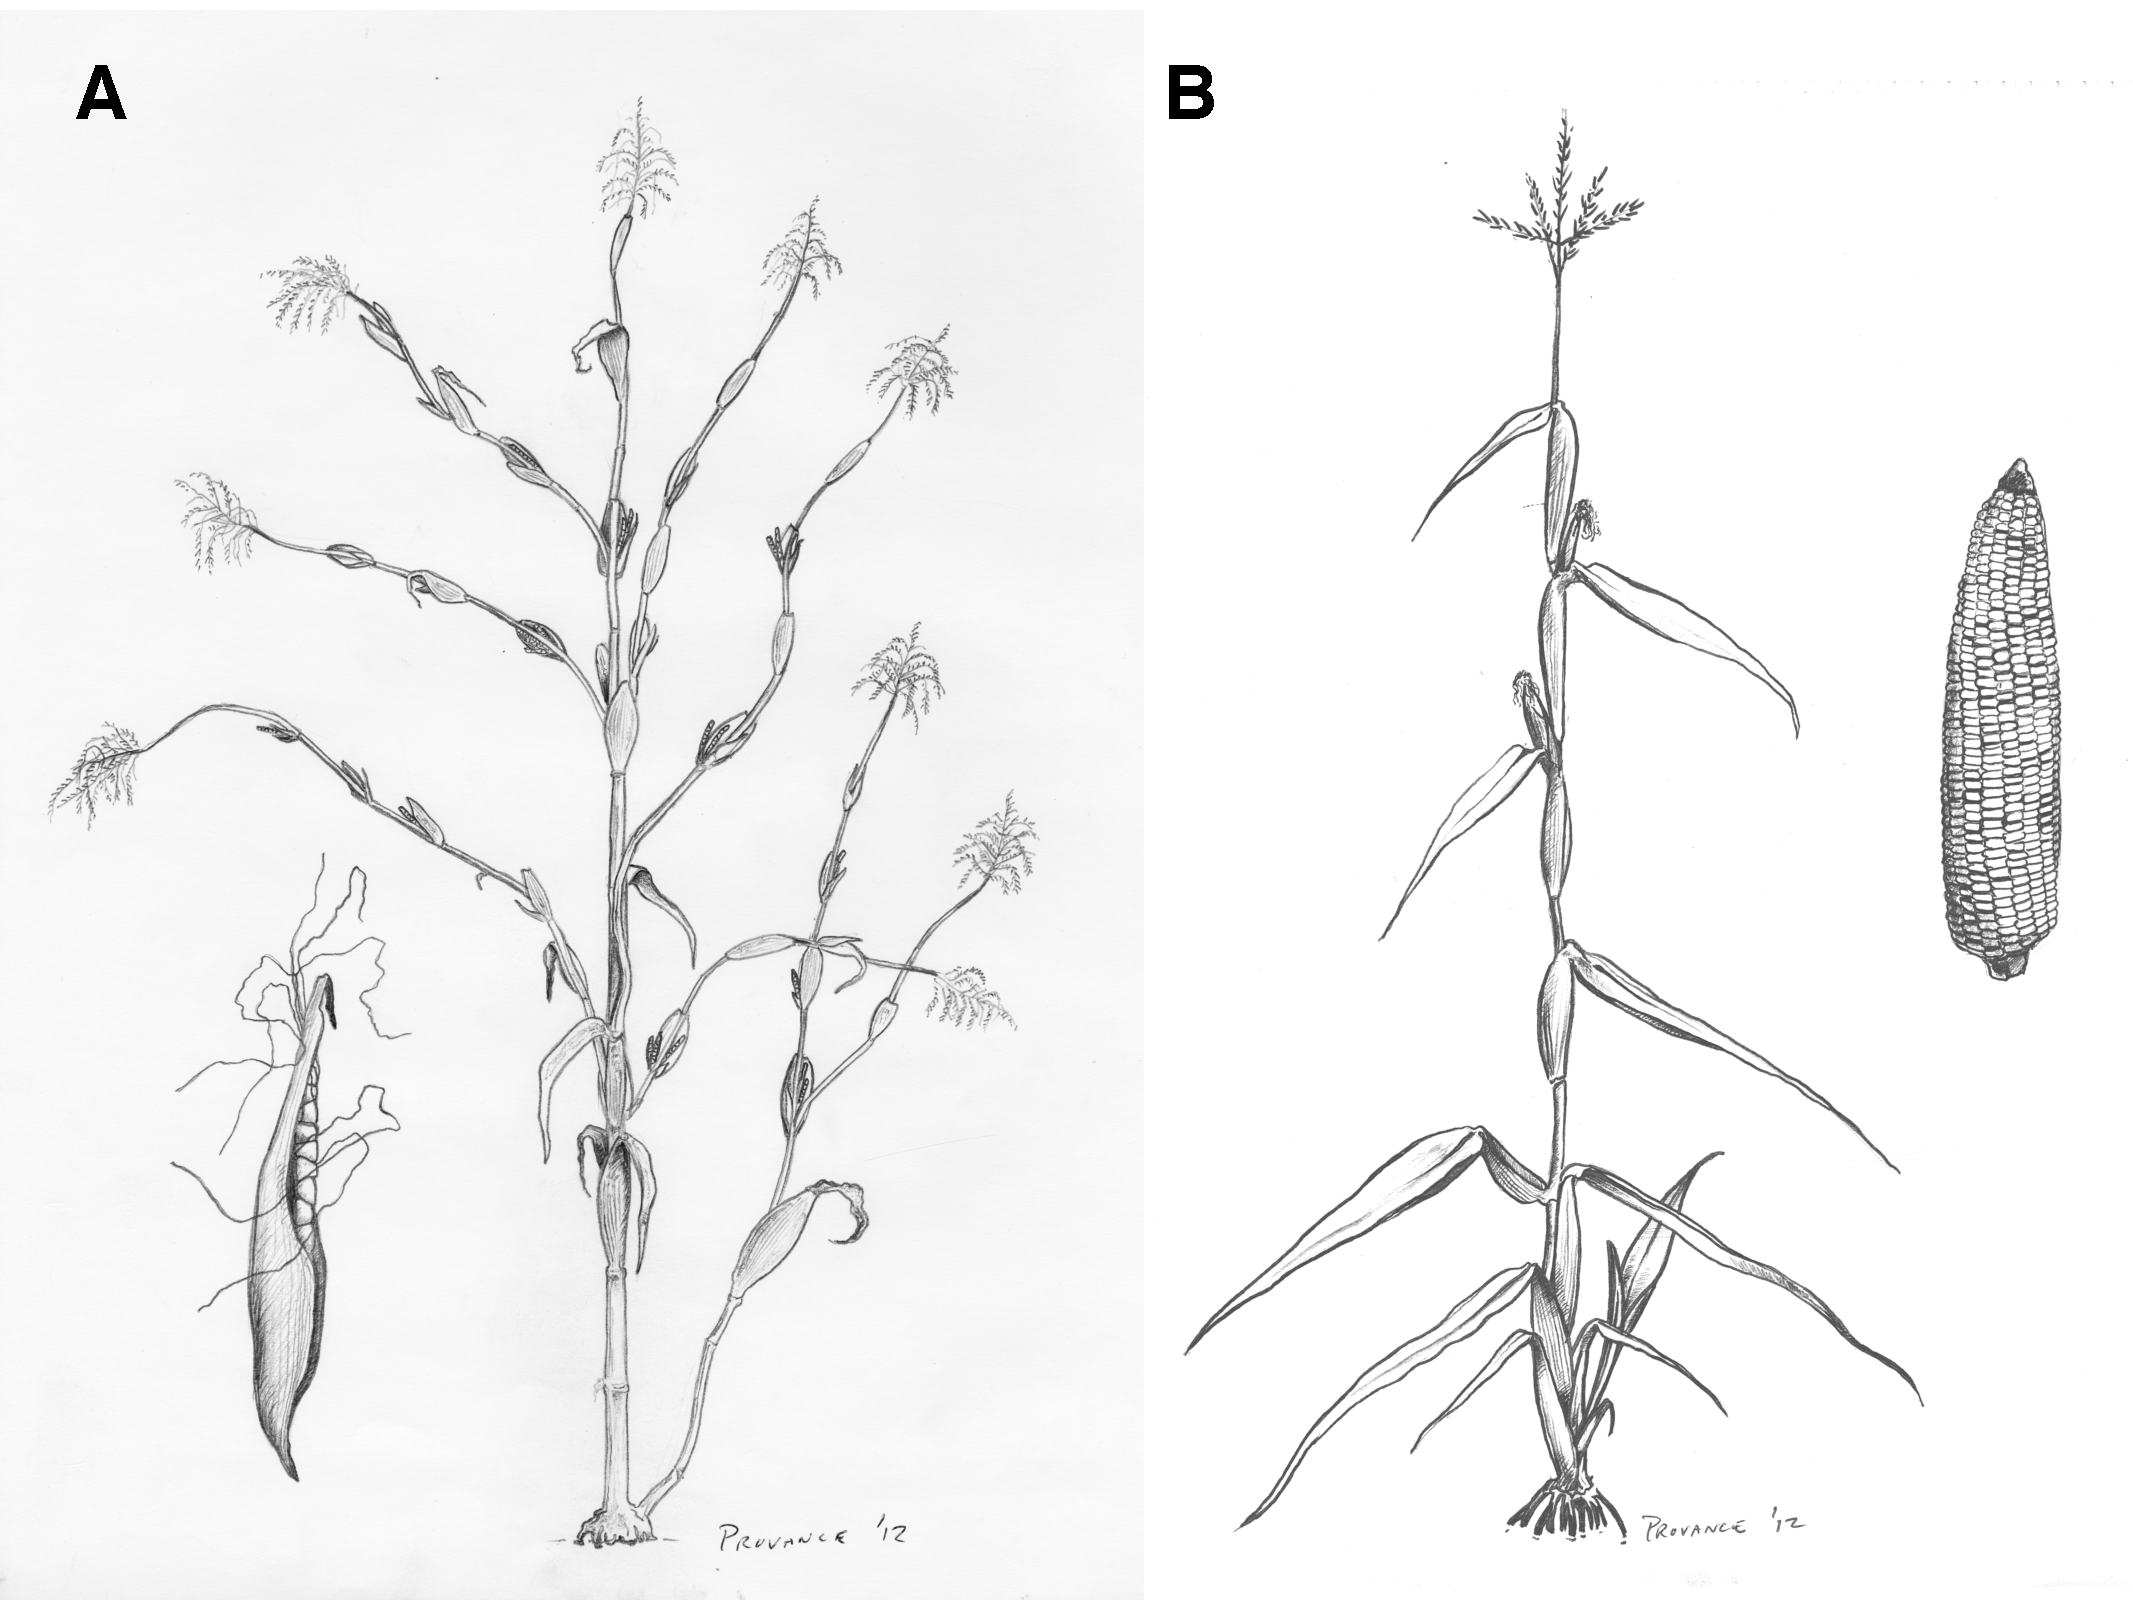
\includegraphics[width=11.4cm, page=1]{figures/maize_teo_plants.pdf}}
        \caption{\label{fig:provance} (A) Teosinte plant architecture is branched, with multiple ears per plant. (B) Maize architecture is apically dominant, with side branches tipped by female inflorescences (ears). }
\end{figure*}



In total, these phenotypes represent the five key morphological differences between maize and teosinte, used in their most recent taxonomic revision \citep{doebley1980, iltis1980}.
A number of other traits distinguish maize and teosinte, many of which can be explained by the premature cessation of growth in axillary branches, leaves, and internodes \citep{doebley1980}.
Other traits involved in domestication, and improvement of maize allowing its worldwide spread include a loss of seed dormancy \citep{avendanolopez2011}, a loss of photoperiod sensitivity \citep{huang2017}, nutritional alterations \citep{hanson1996, whitt2002}, and other phenotypes less apparent than these morphological changes. %\mcs{is this enough improvement?}
Collectively, these phenotypes represent radical departures of maize from \textit{Zea mays} subsp. \textit{parviglumis}, yet both are classified as belonging to the species \textit{Zea mays} in recognition of the continued fertility of these taxa, in the absence of large scale gametophytic incompatibility alleles \citep{kermicle2006}.


\subsection*{Inheritance of phenotypes}


Building on these observed differences between taxa, numerous studies attempted to understand the genetic basis of this differentiation by crossing maize and teosinte to observe phenotypic distributions of these traits in their progeny.
In large part these experiments led to murky conflictions, likely reflecting the use of diverse germplasm, differing quantification of phenotypes, and wide crosses between species with reduced fertility.
This confusion as to the ancestor of maize would not be resolved until molecular methods supported \textit{Z. mays} subsp. \textit{parviglumis} as the direct ancestor \citep{bennetzen2001}, a taxon rarely used in initial investigation.

Early research into maize origins made use of diverse samples of teosinte including \textit{Zea luxurians} \citep{collins1920, rogers1950a, rogers1950b, lambert1965} and  \textit{Zea mays} subsp. \textit{mexicana} \citep{langham1940, rogers1950a, rogers1950b}, and a variety of maize lines such as Tom Thumb popcorn \citep{collins1920}, a photoperiod insensitive maize inbred \citep{rogers1950a, rogers1950b}, maize `of medium maturity' \citep{langham1940}, and Hy2 \citep{langham1940}.
Given our modern understanding of the divergence amonst these teosinte taxa \citep{rossibarra2009} and differences in photoperiod sensitivity among these lines when grown at high latitudes \citep{emerson1924, rogers1950b, wilkes1967}, it is perhaps not surprising that crosses using different teosinte and maize samples produced confounding results.
For example, some studies showed the mature paired spikelets of maize to be controlled by a single Mendelian locus, but others considered the trait to be quantitative, controlled by many genes.
While \citet{rogers1950a} found multiple genes linked to spikelet pairing, he recovered a locus on the same chromosome identified by \citet{langham1940} who considered the trait to be controlled by a single gene.
And when crossing \textit{Zea mays} subsp. \textit{mexicana} to a Peruvian maize variety,  \citet{galinat1959} found F1 ears to contain single mature spikelets, but when the same teosinte was crossed to North American maize, spikelets were paired in the F1 \citep{mangelsdorf1974}.
This shows that a maize allele at one locus cannot be the only gene controlling paired spikelets, without altered dominance in different genetic backgrounds, environmental effects on the trait when grown in different years and locations, or subjective phenotypic classification of the trait by different people.
These differences were likely exacerbated by differences in the number of paired spikelets initiated per whorl, as selection during maize improvement has dramatically increased the number of kernels per row, which may undermine a simple genetic basis.

In total, about half of these studies classified the five major morphological differences between maize and teosinte as quantitative  \citep{collins1920, mangelsdorf1947, rogers1950a, rogers1950b}, while the other half considered them to be controlled by a single Mendelian gene \citep{langham1940, galinat1971, galinat1988}.
And while the original interpretation of both \citet{mangelsdorf1939} and \citet{beadle1939} was that of four major genes or chromosomal regions of linked genes, many later investigations suggested almost every chromosome contributed to the domestication phenotype \citep{mangelsdorf1947, rogers1950a, rogers1950b}.
Viewed from today's perspective, these investigations highlighted 1) that the key morphological differences between maize and teosinte are often oligogenic, 2) that substantial genetic variation exists within both maize and teosinte, 3) that consistent experimental design and environment can alter interpretations, and 4) that the genetic background a maize allele is found in can determine its effect on phenotype.
But, even after observation of tens of thousands of plants across these experiments, the genetic basis of differentiation between maize and teosinte was still unclear, making it difficult to investigate how they evolved and how domesticators selected on them.

\subsection*{QTL mapping beyond single genes}

While connecting the inheritance of individual phenotypes to their underlying genes was complicated by the features discussed above, another alternative was to identify progeny of a F2 population resembling maize and teosinte parents \citep{beadle1972}.
In  contrast to earlier crosses between maize and teosinte, \citet{beadle1972} selected `primitive' maize varieties to avoid confusing genetic variation that was selected during the modern breeding of maize with changes due to domestication.
He grew approximately 50,000 plants of a cross between the maize race Chapalote and his most maize-like teosinte, the Chalco race of \textit{Zea mays} subsp. \textit{mexicana} \citep{beadle1972, beadle1980}.
Approximately 1 in 500 plants yielded ears looking like either the maize or teosinte parent \citep{beadle1972, beadle1980}.
This reduced the number of genes involved to between four and five, similar to that suggested by \citet{langham1940}.
It is notable, however that this observation inherently suggests some deviation from additive gene action --- with four genes, 1 out of 256 plants should have been similar to each parent, and with five genes, 1 out of 1024.

In order to understand the genetic basis of these traits, \citet{doebley1991} repeated this exact cross, phenotyping approximately 250 F2 progeny for domestication related traits but also genotyping each plant.
They identified 58 genomic regions associated with their 12 phenotypes, spread across all 10 chromosomes; most of these, however, were within 5 large regions on chromosomes 1, 2, 3, 4, and 5.
Some phenotypes were controlled by large effect loci, like a single locus on chromosome 2 that explained 77.5\% of the phenotypic variance for the number of kernel rows per ear.
But the majority of associated regions explained less than 10\% of variation, consistent with a more oligogenic or even polygenic architecture.
These researchers extended this work by crossing the presumed direct ancestor of maize, the annual teosinte \textit{Zea mays} subsp. \textit{parviglumis} and the maize race Reventador.
\citet{doebley1993} largely recapitulated their previous results, and identified 50 associations, including some loci only associated in one of their two populations.
Clearly loci that frequently show conditional associations are unlikely to be the key differences between maize and teosinte.
Both studies, however, agreed that these five genomic regions on chromosomes 1, 2, 3, 4, and 5 disproportionately control the phenotypic differences between maize and teosinte, including over 70\% of the loci explaining more than 10\% of phenotypic variance in any trait \citep{doebley1991, doebley1993}.
This overrepresentation was later validated in a larger experiment using backcross progeny of \textit{Zea mays} subsp. \textit{parviglumis} and the inbred line W22 \citep{briggs2007}, in which 64\% of large effect loci were located to these regions. \mcs{progeny of f2? what do you mean}

Foreseeably, these five regions contain major effect loci that differentiate maize and teosinte.
Further research has succeeded in cloning the genes underlying some of these QTL, enabling in some cases identification of the specific mutation underlying phenotypic differences between maize and teosinte.
These genomic regions are presented here in the same order as the morphological traits were introduced.

\noindent They are:


\begin{enumerate}

 \item \textit{The paired spikelets of maize are associated with variants on chromosome 1 and 3 across multiple crosses of maize and teosinte.}
 Over half of phenotypic variation in paired spikelets can be explained by these two loci \citep{doebley1991, doebley1993}, but the interval covers most of chromosome 1 and may represent multiple QTL \citep{doebley1993}.
 These QTL are both epistatic and pleiotropic \citep{doebley1995}, with altered allelic effects in maize versus teosinte backgrounds, and impacting many other traits like plant architecture.
 Other loci are associated with paired versus single spikelets, notably those on chromosomes 2, 4, and 10 \citep{doebley1991, doebley1993}. %\mcs{fine to remove this sentence, but helps later with genes}
 Some genes underlying spikelet formation are known from developmental genetic screens (\textit{ramosa1} (\textit{ra1}), chromosome 7; \textit{ramosa2} (\textit{ra2}), chromosome 3; \textit{ramosa3} (\textit{ra3}), chromosome 7) \citep{vollbrecht2005, mcsteen2006}, but these do not fall into the QTL intervals identified in these crosses.
 Presumably, these genes are members of pathways involving genes in these QTL, as \textit{ra1} controls the switch to inflorescence determinacy that occurs with the production of spikelet pairs \citep{vollbrecht2005}, and shows evidence of selection during domestication \citep{sigmon2010}.
Fine-mapping the loci distinguishing paired and single spikelets is complicated by difficulty in phenotyping paired spikelets, as their appearance can be difficult to identify given the high number of kernels in each row of the ear of modern maize parents \citep{galinat1988}.


 \item \textit{The two ranks of the teosinte ear are largely controlled by the gene \textit{Zea floricaula leafy2} (\textit{zfl2}) \citep{bomblies2006}. }
 This gene is responsible for reproductive identity, forming multiple ranks along the inflorescence meristem.
 \textit{zfl2} is found within a QTL interval on chromosome 2 that explains 36-77.5\% of phenotypic variance for the number of rows of cupules \citep{doebley1991, doebley1993}, and the gene itself explains 9\% of variation in ear rank number across multiple maize-teosinte mapping populations that have an intact or mutant version of the maize allele \citep{bomblies2006}.
  There are additional QTL on chromosomes 1, 3, 4, 5, 9, and 10  that modify this phenotype \citep{doebley1991, doebley1993, briggs2007}, including a paralog, \textit{Zea floricaula leafy1} (\textit{zfl1}), on chromosome 10 \citep{briggs2007} which may alter the effect of \textit{zfl2} \citep{bomblies2006}.

 \item \textit{The disarticulating rachis of the teosinte ear are controlled by alleles at \textit{ZmSh1-1}%/yabby homolog10} (\textit{yab10}),
 and \textit{ZmSh1-5.1+ZmSh1-5.2}%/C2C2-YABBY-transcription factor 6} (\textit{yab6})
 , although variation within teosinte identifies \textit{Zea agamous-like1} (\textit{zagl1}) to be a candidate.}
 This trait was ascribed to various loci that explained high amounts of phenotypic variation in crosses using different teosinte parents \citep{doebley1991, doebley1993}, and association mapping within teosinte identifies \textit{zagl1} as a potential candidate \citep{weber2008}. %\mcs{this weber not enough?}% in a region that explains 25.8\% of variation in one maize cross \citep{doebley1991}.
Within maize, tandem duplicates of a ortholog of \textit{shattering 1} (\textit{Sh1}) on chromosme 5 explain 23.1\% of variation in shattering \citep{lin2012}, and maize alleles at \textit{ZmSh1-1}, a transcription factor associated with shattering in other grasses \citep{lin2012}, elongate internodes via an epistatic interaction with \textit{tb1}\citep{yang2016}. %%new addition - check that makes sense!
 \textit{zagl1}, a MADS box transcription factor, is associated with ear size and has pleiotropic effects on flowering time \citep{wills2017}, but is unlikely to be the only locus involved in ear disarticulation.

 \item \textit{Although many ear traits differ between maize and teosinte, the most dramatic one observable in crosses is that of hardened glumes, controlled by the gene \textit{teosinte glume architecture1} (\textit{tga1}).}
 The maize allele of \textit{tga1} inhibits secondary sexual traits in the female flower, preventing glumes from hardening \citep{preston2012}.
 A nonsynonymous mutation in exon 1 of \textit{tga1} alters dimerization of the protein, affecting its stability and preventing activation of downstream targets \citep{wang2015}.
 The chromosome 4 QTL that contains \textit{tga1}  explains between 27-62.4\% of phenotypic variation for glume hardness \citep{doebley1991, doebley1993, briggs2007}.
% This appears to be the biggest effect gene, where one major gene disrupts the infructescence, making it more male like.
 Additionally, this gene appears to have pleiotropic impacts on disarticulation, lateral branch length, the pedicilate spikelet, and phyllotaxy \citep{wang2015}.

 \item \textit{Aside from ear traits, the clearest morphological difference between maize and teosinte is plant architecture, for which
 \citet{doebley1995} first identified \textit{teosinte branched1} (\textit{tb1}) as the major locus. }
 The QTL region \textit{tb1} is found within explains 35.9\% of variation in the number of basal branches or tillers \citep{doebley1991}.
 Later efforts identified the precise causal muation: rather than a change in the coding sequence of the gene, a transposable element insertion 65 kb upstream of the gene appears to enhance expression of \textit{tb1} \citep{studer2011}.
 This increased expression represses lateral branching, allowing the primary lateral inflorescence to compress into a female structure.
 The locus is allelic to a maize mutant that generates a branched, tillered phenotype \citep{burnham1959}, and other loci within the QTL are pleiotropic for ear architecture traits \citep{studer2011fract}.
 Other genes involved in plant architecture were selected during domestication, including \textit{grassy tillers 1} (\textit{gt1}), where the maize allele reduces the numerous small ears found in teosinte to a limited number of large ears \citep{wills2017}.


 \end{enumerate}


Larger studies focusing on QTL for similar morphological traits identified 314 QTL for 22 traits involved in domestication and improvement \citep{briggs2007}.
But only 14 of these explained more than 10\% of variation in a trait, which overlap (almost) perfectly with QTL regions shown to be major domestication QTL \citep{doebley1993}.
Some traits could be explained by only six QTL, while others required 26, but low-oligogenic traits were mostly for improvement post-domestication.
Together, this suggests that while these major regions are important for domestication, many other genes in the genetic background contributed and modulated these phenotypes.

\subsection*{Maize domestication involved many loci}

\citet{mangelsdorf1974} attempted to reconstruct a teosinte phenotype by moving the four major segments he identified as important for a maize phenotype from teosinte into a single maize inbred line.
This did not work, instead generating a plant indistinguishable from maize.
However, selective breeding of a teosinte plant with maize ancestry rapidly turned a teosinte-like phenotype to maize in only 18 years \citep{weatherwax1924, collins1925}, suggesting segregating alleles can be selected to reconstitute the maize phenotype.
While the handful of regions discussed above can have large phenotypic effects, it clearly takes more than five genes to make a maize plant.
\citet{briggs2007}, in large crossing experiments between maize and \textit{Z. mays} subsp. \textit{parviglumis} identified 314 QTL, of which only 14 explained more than 10\% of variance for any trait.
Only approximately 50\% of total phenotypic variation in all traits could be explained by the identified QTL \citep{briggs2007}, leaving a large amount of unexplained variance, presumably attributable to environmental differences, epistatic relationships, or small QTL that may become statistically observable with differing experimental designs \citep{yu2008}.

In contrast to QTL approaches focused on identifying the genetic basis of specific phenotypes, a number of population genetic studies have scanned the genomes of maize and teosinte for signs of natural selection, such as reduced nucleotide diversity around selected genes.
Selection scans can identify loci important for fitness beyond those underlying morphological differences associated with domestication, like loci involved in response to biotic or abiotic environments.
Analyses of microsatellite diversity \citep{vigouroux2002, vigouroux2005} and sequence data from hundreds of individual loci in teosinte and inbred maize lines \citep{wright2005} both suggested that 2-5\% of the genome had been targeted by selection.
Whole-genome resequencing of teosinte and traditional maize landraces found a similar proportion of the genome affected by selection, identifying 484 regions as outliers, each likely representing a gene under selection during domestication \citep{hufford2012natgen}.
Together, these studies suggest that a substantial proportion of the maize genome has been selected during domestication.
As selection during domestication occurred during a relatively short period of time, compatible interactions between many loci were required for phenotypes to shift.


 \section*{The tempo of maize domestication}

Knowledge of individual alleles that were selected during domestication allows investigation into the time these alleles arose and how selection acted to increase their frequencies.
Archaeological and molecular methods agree that maize was domesticated 9000 years ago in the seasonally wet lowlands of the Balsas Valley of Mexico (Figure \ref{fig:map})  \citep{matsuoka2002, piperno2009, ranere2009}.
Although macrobotanical maize remains from the region have not been found, likely due to the poor conditions for preservation, phytoliths from cobs support the emergence of \textit{Zea mays} subsp. \textit{mays} in this region \citep{piperno2009}.
The first macrobotanical remains morphologically characterized as maize come from the dry highlands 6,200 years before present \citep{mangelsdorf1967, benz2001, piperno2001}.
Morphological intermediates are rare in the archaeological record, reflecting a rapid transition from a teosinte-like phenotype to a maize-like phenotype.
In the earliest archaeological samples of maize, cobs are non-disarticulating, have softened glumes with a narrow rachis, and shallow cupules with evidence of one or two spikelets \citep{mangelsdorf1974, benz2001,  kennett2017}.

Early genetic \citep{jaenickedespres2003} and recent genomic  \citep{fonseca2015,  ramosmadrigal2016, vallebueno2016, swarts2017} investigation of archaeological samples integrate morphology and genotypes at known domestication loci.
A reduction in diversity around \textit{tb1} in all archeaological samples indicates that the maize allele was present, suggesting this allele rapidly increased in frequency.
The maize allele at \textit{tb1} arose 28,000 years before present \citep{studer2011}, and is found segregating at frequencies up to 44\% in teosinte populations \citep{studer2011, vann2015}.
That the allele was present before domestication, and does not always generate a maize-like phenotype when present in teosinte \citep{vann2015} shows that knowing this maize allele is present is not enough to generate a maize-like phenotype. \mcs{knowledge is not what matters, say what you mean}
In contrast, the maize allele at \textit{tga1} that restructures glumes and cupules of the ear was fixed within the last 10,000 years \citep{wang2005}, likely a result of selection on a new non-synonymous mutation \citep{wang2015}.
Of the two oldest cob samples sequenced, \citet{ramosmadrigal2016} find the maize allele at \textit{tga1}, while \citet{vallebueno2016} do not recover the causal polymorphism, but find elevated diversity in the region, which they suggest reflects incomplete selection on the maize allele.
Consistent with rapid selection after mutational origin, no phenotypes resembling the effect of a mutation at \textit{tga1} were observed when George Beadle examined more than 2 million teosinte seeds from a number of wild populations  \citep{beadle1980, bergsingerbook}.
Mutations that alter the fruitcase were thus likely rare or absent in teosinte populations, and presence of the maize allele in archaeological samples is consistent with rapid fixation during during domestication.

In order to ascertain the presence of a maize allele in a teosinte population, and identify when selection acted, the functionally relevant causal variant must be identified.
Unfortunately, \textit{tb1} and \textit{tga1} remain the only loci selected during maize domestication for which this level of detail is known.
Outside of the alleles at \textit{tb1} and \textit{tga1}, only the \textit{gt1} locus has been investigated in this manner, with a maize allele that arose 13,000 years ago, and is found segregating at low frequencies in teosinte \citep{wills2013}.
Their contrasting patterns --- from segregating variation found today in teosinte (\textit{tb1} and \textit{gt1}), and from a new \textit{de novo} mutation (\textit{tga1}) --- cannot be generalized without further research into the causal alleles of maize domestication. \mcs{contrasting pattern exists, more study will not erase it, you don't say what you mean}

The presence of standing variation can accelerate the speed of evolution when selection pressures shift.
Rather than waiting for a mutation that generates a phenotype, the presence of both genetic and phenotypic variation allows rapid selection.
This drpends on how deleterious a mutation is --- which can be affected by its dominance, epistatic interactions with other alleles, and its pleiotropic effects on other traits.
Hence, it is important to integrate these alleles not independently, but in aggregate with everything else in the maize genetic background. \mcs{this does not mean what you mean to say}

\section*{Genetic interactions and selection during maize domestication}
\subsection*{Shifting dominance of domestication alleles in maize}

Dominance, or interaction between alleles at a single locus, affects the exposure of an allele to selection.
Although dominance modifiers can evolve, the recessivity of new mutations seems to be a general feature \citep{orr1991}.
Dominance is informative as to how selection could act on new mutations, and relevant to thinking about the visibility of segregating variation to selection.
As the alleles present at a locus vary between individuals, dominance can alter the phenotypic outcome of different crosses.

In \textit{Zea mays}, the dominance of a given allele can differ based on its genetic background.
When QTL carrying a maize allele from chromosome 1 or 3 were introgressed into a teosinte background, the maize allele was on average recessive to the teosinte allele in its effect on seven different phenotypes \citep{doebley1995}.
But when a teosinte allele at either locus was introgressed into a maize background, the maize allele was partially dominant to the teosinte allele, an effect also seen when segregating in a F2 population \citep{doebley1995}.
Dominant maize-like alleles arising in a teosinte background may be rapidly selected against, as if a maize-like phenotype arises in teosinte, it will be detrimental to plant fitness.
And as the alleles we today denote as `maize' initially arose in a largely teosinte background, their dominance measured today in maize  may not reflect that they first experienced.
If this recessivity of new `maize' alleles is general to domestication loci, alleles could survive with relaxed fitness costs until human selection increased their frequency \citep{doebley1995, lauter2002}.

Although the dominance of these two QTL have been most extensively studied, other evidence exists for the recessivity of maize alleles in a teosinte background and their impacts on human selection.
The maize allele of \textit{tga1} is dominant to the teosinte allele, reducing deposition of silica in glumes \citep{dorweiler1997}.
In a maize background, the teosinte allele of \textit{tga1} decreases grain quality, because kernel growth is restricted by the hardened glumes, leading to cracking and susceptibility to pathogens \citep{dorweiler1993}.
But the maize allele of \textit{tga1} likely arose in a teosinte genetic background and the effect of the maize \textit{tga1} allele in a teosinte background is less detrimental.
Although ears of such a plant are shorter, they are still protected within husks until harvest \citep{dorweiler1993},  and although mature kernels are exposed to pests, cultivation practices can ameliorate such danger.
This phenotype of the maize allele in a teosinte background could allow visual identification of heterozygotes \citep{wang2005}, yet none were identified in a screen of more than 2 million teosinte seeds \citep{beadle1980, wilkes2004, bergsingerbook}.
Consistent with this, the maize allele appears to have arisen \textit{de novo} during domestication  \citep{wang2015}, suggesting  the necessity of human cultivation to select for this dramatic phenotype.

Beyond single loci, the phenotypic means in F2's of maize $\times$ teosinte crosses and backcrosses of teosinte to maize deviate towards the teosinte parent \citep{lambert1965, doebley1990, doebley1993,  doebley1995}.
While some of these results could reflect epistasis, it nonetheless suggests that for a substantial portion of the genetic background, the teosinte allele is dominant in a teosinte background --- most similar to the genomic environment an allele would be selected in.  %\jri{as soon as you are in bc1 the background is now more maize than teosinte, so not sure that makes sense. also seems here you're arguing inf avor of Haldane's sieve where above you were making the Orr/Betancourt argument against?} \mcs{these are modern alleles? the background is a majority maize, but we're thinking about dominance here, not epistasis. BC1 means all teo alleles that are present are in hets, so suggests some dominance to me. Could be more explicit with the numbers and d/a ratios in BC's but I don't think it is worth it.}%\mcs{not clear to be dominant in what bkgd on this para}
%\jri{but text says bc1 shows evidence teo alleles are dominant int a b a teo background. but bc1 only shows teo allele dominant in maize background (and F2's should be on expectation 50/50)... that's where i'm lost.}

Another way to consider dominance is through the molecular phenotype of gene expression.
Transcriptome-wide, 52-58\% of genes have maize alleles that are more highly expressed than teosinte alleles \citep{hufford2012natgen, swansonwagner2012, lemmon2014eqtl, wang2017}, which may result from selection for consistent expression across changing environments \citep{doebley1995, lorant2017}.
Further, this pattern is intensified in domestication candidate genes, with 60\% of candidate genes showing higher expression of the maize allele \citep{hufford2012natgen, swansonwagner2012}.
In allele-specific expression studies of crosses between maize and teosinte, the maize allele of genes with \textit{trans} regulatory control are more commonly dominant to the teosinte allele in ear and leaf tissue,  %\mcs{this doesn't feel right as written, revisit}
consistent with a contribution of dominant transcription factors and expression modifiers by the maize parent \citep{lemmon2014eqtl}.
The effect is not subtle, with 70-80\% of genes showing dominance of the maize allele \citep{lemmon2014eqtl}.
Both dominance of expression and higher expression in maize may reflect selection for robustness of expression in the face of differing environmental conditions, assuring fitness under cultivation \citep{doebley1995}.
%\jri{not sure what this argument is. why does high expression = robust to changing environment? happy to discuss}\mcs{changing environment changes gene expression to respond. not changing gene expression makes phenotype more robust to a changing environment. there are physiological barriers and thresholds so higher is more robust.}\jri{your call, but i'd drop this. i don't understand/buy this argument, but if it's clear to you and i'm just misunderstanding, please keep it in and remind me so you can explain to me later.}

Although maize alleles are dominant to teosinte alleles in a maize background, dominance relationships shift when alleles are segregating in an F2, a teosinte backcross, or a maize backcross \citep{doebley1995, briggs2007, doust2014}.
This suggests that interactions among loci --- perhaps many loci --- can alter the efficacy of selection on a particular trait.

\subsection*{Epistasis}

Epistasis can be envisioned in numerous ways, but we highlight two extremes.
Statistical epistasis refers to deviations from additive relationships in a model \citep{fisher1918}, while biological epistasis describes the interaction of gene products \textit{in vivo} \citep{bateson1909}.
The two can be difficult to distinguish with experimental data, because, for example, it is impossible to identify stastistical epistasis for a locus exhibiting biological epistasis if the experimental population lacks variation for one interacting gene partner.

In maize, statistical epistasis is rarely observed in QTL analyses \citep{edwards1987, stuber1992, briggs2007} or in genome-wide scans in panels of inbred maize lines \citep{wallace2014} (but see \citet{shi2016} for epistatic effects in leaf orientation), but is more commonly found when individual cloned QTL are placed into otherwise isogenic maize or teosinte backgrounds \citep{doebley1995, weber2008,  studer2011fract}. %especially when using teosinte
As variation both in the genotype and phenotype of a causative locus must occur in a mapping population, studies focusing on maize specifically may fail to observe differences.
A lack of genetic variation may not be due solely to selection having removed it ---  the genetic bottleneck arising from maize domestication altered allele frequencies throughout the genome \citep{eyrewalker1998,tenaillon2004, wright2005, beissinger2016}, and modern maize often lacks phenotypic variation for relevant traits \citep{briggs2007, xue2016, xu2017}.
Statistical epistasis thus may not exist in most mapping populations and experiments.
Consistent with this argument, statistical epistasis is identified with comparable ease in QTL populations that include a teosinte parent \citep{weber2008}, although this does not always ameliorate the issue of limited allelic input.
For example, \textit{zfl2}, the locus controlling ear phyllotaxy, was not recovered in a backcross of \textit{Zea mays} subsp. \textit{parviglumis} to inbred maize \citep{briggs2007}, complicating the interpretation of this major effect locus.

%\jri{is http://www.genetics.org/content/genetics/67/1/137.full.pdf relevant for this section? the discussion there is good.} \mcs{have not read, will}

While insufficient variation at the loci involved is likely at least partly responsible for discrepancies among studies, the design of mapping populations can also dramatically impact the power to detect different forms of epistasis.
Because of the large number of potential combinations and the need to control for genetic background,
very large experimental populations are needed to test for statistical epistasis, and often only the strongest effects can be identified.
Indeed, by phenotyping seven times more progeny than earlier mapping studies of maize and teosinte, \citet{briggs2007} identified 29 two-locus epistatic interactions, although only one was found in both environments studied.

In addition to sample size, the kinds of crosses made will determine what allelic variation is present that could be scored as epistasis.
For example, in an F2 between maize and teosinte, the combined additive and epistatic effects of two QTL, on chromosomes 1 and 3, explain 60\% of variation in paired vs. single spikelets \citep{doebley1995}, but when these regions are introduced into a teosinte background via backcrossing they explain only 7.3\% of variation in this phenotype.
This suggests that numerous other genes in the genetic background interact to generate this phenotype and supports earlier experiments that found different numbers of loci controlling the trait in progeny from different crosses \citep{langham1940, szabo1996}.

During domestication, epistatic variation may be converted to additive variation, as alleles fix at one or more of a set of interacting loci.
But during intermediate phases after an allele arises but before selection fixes it, epistasis may alter the efficacy of selection.
This can be seen in the interaction between QTL on chromosomes 1 and 3.
When the frequency of the maize allele of the chromosome 1 QTL is low, the chromosome 3 QTL has little effect on the proportion of branches terminated by male inflorescences, a teosinte-like trait \citep{doebley1995}.
But when the chromosome 1 allele containing \textit{tb1} increases in frequency, the ability to select on its interacting partner on chromosome 3 increases, as this epistatic variance increases at intermediate allele frequencies \citep{goodnight2004}.
With both teosinte alleles in a maize background, terminal inflorescences are 90\% male, but by simply substituting either QTL, this proportion is reduced to 21\% with a teosinte allele at chromosome 1 or 0.5\% with a teosinte allele at chromosome 3 \citep{lukens1999}.
The recent characterization of the candidate gene \textit{tassels replace upper ears1} (\textit{tru1}) within the chromosome 3 QTL \citep{dong2017} and additional candidates within the chromosome 1 QTL \citep{yang2016} may allow finer scale temporal tracking of allele frequencies and the role of selection on epistatic partners.%\jri{not sure this sentence is needed?}
It appears that both the phenotype presented to selection and the response to selection are dependent on other loci in the genome.
Although the statistical power to detect epistasis may be poor, such examples of biological epistasis may be common.
For example, much of the shade avoidance pathway downstream of \textit{tb1} has been shown to be targets of selection \citep{studer2017}, but these are not detected in screens for statistical epistasis. \mcs{the noun is pathway which is singlular so the sentence needs to be fixed}
Together, despite the fact that few loci have shown evidence of statistical epistasis in mapping studies, there is evidence for epistasis --- both statistical and biological --- contributing to domestication.


In total, these epistatic effects and the importance of the genetic background may alter the course of selection on phenotypes.
If buffered by their interaction with other genes, maize alleles could have been maintained in wild populations of teosinte with little effect on phenotype or fitness.
Indeed, a number of experiments in teosinte have demonstrated the existence of such cryptic variation for maize-like traits \citep{lauter2002, weber2007, weber2008, vann2015}.
The introduction of new variation --- via new mutations or hybridization between populations --- could then release cryptic epistatic variation, generating novel phenotypes \citep{doebley1995}.

\subsection*{Pleiotropy}

Pleiotropy describes the effect of an allele of a gene on seemingly unrelated phenotypes.
It can constrain the path of evolution, as directional selection on a phenotype can be limited if the allele has deleterious effects on another phenotype, or facilitated if the allele has beneficial effects on fitness in different life stages.
Alleles that are more pleiotropic are more likely to negatively impact at least one other trait \citep{fisher1918}.
Understanding pleiotropy and the correlation of phenotypes can help to understand constraint on the outcome of selection.

But pleiotropy  can be confusing, as phenotypes that appear superficially different may not be truly distinct.
Plants are constructed of repeated units of leaf, stem, and bud, known as phytomers.
The genes involved in generating these phytomers thus can be readily pleiotropic via development, having an effect on phenotypes that may appear at first glance distinct.
In light of the phytomer, it is not entirely surprising that pleiotropic loci explain correlation in developmental traits of ear and tassel \citep{brown2011}, flowering time in male and female flowers \citep{buckler2009}, or leaf length and flower length \citep{tian2011}.
But pleiotropic loci extend even beyond the phytomer, as QTL involved in tassel and ear development are also classified as flowering time genes \citep{xu2017}.
In many such studies, it is not yet clear how many genes contribute to the observed pleiotropy, as efforts to fine-map individual QTL can split effects within the region into multiple heritable loci \citep{lemmon2014dissect}.


Understanding pleiotropy and the correlation of phenotypes can help to understand constraint on the outcome of selection.
For example, the maize allele at \textit{zfl2}, is implicated not only in the spiral ear phyllotaxy that generates increased kernel number but also in a number of traits including earlier flowering \citep{bomblies2006}. %earlier flowering, more ears, and more maize-like internodes \citep{bomblies2006}.
But in an environment that maize flowering time is well-adapted to, stabilizing selection on flowering time might limit the response to directional selection for increased kernel number. \mcs{i don't think you mean to say that flowering time is well adapted}
Hence, such pleiotropy may constrain domestication alleles when selection axes disallow variation.
For example, if selecting for increased kernel row number was accompanied by an acceleration of flowering time to values too early for current environmental conditions, this correlated selection may limit response to selection for increased kernel number.

It has long been noted that many of the loci that differentiate maize and teosinte are pleiotropic \citep{collins1920, beadle1939, mangelsdorf1939, langham1940}.
Recent dissection of the regulatory architecture of \textit{tb1} provides a detailed understanding of pleiotropy for a single domestication gene.
\textit{tb1} is pleiotropic across many traits --- apical dominance, length of lateral branches, growth of leaves on the lateral branches, pedicillate spikelet development, and root architecture \citep{hubbard2002, gaudin2014}.
As a transcription factor, \textit{tb1} binds to many regions of the genome.
It directly regulates \textit{tga1} by binding its promoter but is also intimately linked to the cell cycle as it represses two cell cycle genes (\textit{proliferating cell nuclear antigen2}(\textit{pcna2}) and \textit{minichromosome maintenance2/prolifera} (\textit{mcm2/prl})) \citep{studer2017}.
Beyond \textit{tb1}, other loci within the QTL region on 1L found by multiple studies \citep{doebley1991, doebley1993, briggs2007} contribute to ear morphology \citep{studer2011fract, yang2016}, suggesting pleiotropy is common.
%The presence of pleiotropy can constrain how selection acts, and the radical restructuring of the maize ear independent from vegetative structures may reflect this transition. %\jri{i don't understand this. first, what transition? second, it seems that radical restructuring of X independent of Y implies no pleiotropy doesn't it?} \mcs{my argument is that there is tons of pleiotropy within the ear, but it is somewhat removed from the rest of the plant, by these modular network connections}

The presence of pleiotropy creates genetic correlations among traits, potentially constraining the action of selection. \jri{tweak?}
Perhaps because of this kind of constraint, the only mutation thought to have arisen \textit{de novo} and rapidly fixed during domestication is the nonsynonymous substitution in \textit{tga1}.
While the \textit{tga1} ortholog in rice has pleiotropic effects on inflorescences and vegetative structures \citep{preston2012, wang2015}, \textit{tga1} is expressed only in the maize ear, likely a result of gene duplication of an ancestral single locus, with subsequent subfunctionalization  restricting expression to the ear \citep{preston2012, wang2015}.
The paralogous locus, \textit{not tga1}(\textit{not1}), retains expression profiles as found in other grasses \citep{wang2011, wang2012}, suggesting that in maize, the effects of the maize allele of \textit{tga1} are limited to the fruitcase itself, freeing it from constraints on selection imposed by pleiotropic effects elsewhere in the plant.

%Hence, much of the ear of maize can be generated by this direct interaction, and incorporating these interacting alleles into a unified genetic background.

% \subsection*{Plasticity and genotype by environment interactions}
%
% Environmental variation in phenotype may also explain some of the contrasting results found in many mapping studies.
%  %effects on phenotypeallele may not recapitulate similar results is interactions of that allele with environmental conditions.
% Plasticity is the response of an individual genotype to an environment, such that observed phenotypes are reflective of the environment currently experienced or experienced during development.
% Variation in plasticity among genotypes, termed genotype by environment interactions, can restrict how selection acts on a phenotype.
%
% The maize tb1 allele shows reduced response to environmental conditions.
% Although often considered first for its role in maize phenotypes (its name comes from the mutant teosinte branched 1), the tb1 gene is involved in the environmental sensing pathway of shade responsiveness, where it aggregates signals of light and stress \citep{doebley1995}.
% When teosinte plants are exposed to different stressors (e.g. shade \citep{doebley1995} or  low CO2 \citep{piperno2015}), they respond by reducing lateral branching.
% Thus, apically dominant maize has assimilated the stress responsive phenotype, and the allele has lost responsivity to environmental cues.
% This is due to loss of sensitivity to upstream signals from the the shade avoidance network \citep{studer2017}.
%
%
% Cooption of existing networks and modules during domestication may be a common theme.
% In maize, the phase change from the juvenile phase to adult is mediated by the microRNA corngrass1 (miRNA156) \citep{chuck2007}.
% This microRNA targets tga1 \citep{chuck2007}, uniting phenotypic modules of the juvenile-adult transition and ear morphology.
% Assimilation of gene expression in maize relative to teosinte \citep{lorant2017} may also reveal less sensitivity of domesticated alleles to environment --- from the environment the plant is in, to the cellular environment the gene product of an allele is in.
% And in regions of the genome selected during maize improvement and adaptation to various environmental conditions, plasticity is reduced \citep{gage2017}.
% This is consistent with overall findings that crops show reduced plasticity relative to their wild relatives \citep{harlan1992}, where selection for loss of plasticity may allow more consistent and predictable harvest.


\section*{Gene networks of maize domestication alleles}



The molecular basis of pleiotropy may occur when key genes in regulatory networks alter different downstream targets, affecting different pathways.
Selection on correlated traits during domestication could act through a single mutation to a node in a regulatory network, if the trait correlation is due to the network.
 MADS box transcription factors are overrepresented as showing evidence of selection during maize domestication as compared to random genes \citep{zhao2011}.
In plants, MADS box transcription factors are disproportionately represented in the pathways specifying floral organs \citep{theissen2001}, and several MADS box genes are directly regulated by either \textit{tga1} or \textit{tb1} in maize \citep{wang2015, studer2017}.
As one of the biggest alterations in the transition from teosinte to maize is the floral morphology of the ear, the pleiotropic consequences of downstream targets of key domestication genes seem to be involved.
By targeting floral-organ genes, pleiotropic outcomes can be limited in morphological scope, from the shape of the rachis to changes in lignification and silica deposition in the glume and rachis \citep{doebley1996, dorweiler1997}.
Indeed, with the exception of \textit{tb1}, many alleles selected during maize domestication only altered ear morphology.
Selection during domestication can amplify the impacts of alelles through pathways and networks, generating more extreme visible phenotypic outcomes, often intensified by dominance and epistasis.

But networks are not limited to the ear.
Although recovery of spontaneous maize mutants has been one of the most useful features of maize as a model genetic organism \citep{strable2009, nannas2015}, relating phenotypes from such alleles to natural variation can sometimes be misleading.
Spontaneous mutant phenotypes that make a maize plant look more like teosinte are common (e.g. \textit{suppressor of sessile spikelets1}(\textit{sos1}) \citep{doebley1995sos1}, \textit{barren stalk1} (\textit{ba1}) \citep{gallavotti2004}, \textit{tru1} \citep{dong2017}, \textit{tunicate1} (\textit{tu1}) \citep{wingen2012}, \textit{corngrass1} (\textit{cg1}) \citep{chuck2007}).
Upon detailed analyses, however, alleles of these loci often do not show population genetic signatures of selection during domestication and lack functional differentiation between the maize and teosinte alleles.
That large effect hubs of gene networks are frequently observed as the target of selection, producing genetic redundancy in generating phenotypes,  by impacting different stages in pathways or positions in networks, generating an important role in domestication. %, indicates that the large effect domestication loci observed frequently as targets of selection represent large effect hubs of gene networks.
\mcs{recheck, anne is right}

\mcs{this next paragraph is confusing}
Efforts to unite domestication loci into pathways and networks have elucidated the targets of selection.
In contrast to the largely background-specific effects of many maize alleles, \textit{tb1} remains robust to genetic background --- so much so that tillering was not phenotyped in F2 crosses beyond initial work by \citet{doebley1991}.
That  \textit{tb1} was so routinely implicated in differences between maize and teosinte may be true because it has an effect in every population tested thus far and because it is near the top of the shade avoidance pathway \citep{studer2017}.
Consequently, phenotypic effects can be amplified and fine-tuned through downstream targets.
Additionally, several downstream targets of \textit{tb1} show signatures of selection \citep{studer2017}, suggesting further constraint on the entire pathway.

\section*{Implications of gene interactions on evolution and selection}

Investigation into domestication is by definition retrospective --- we are attempting to reconstruct how selection acted to generate phenotypes observed today.
But an understanding of the importance of genetic interactions, including dominance, epistasis, and pleiotropy --- and how they have complicated dissection of even simple phenotypes may provide guidelines for future efforts seeking to identify the genetic basis of phenotypic variation.
That genetic background can impact phenotype is not a surprise, for example, as textbook examples of epistasis include anthocyanin genes in maize kernels \citep{coe1988}.
But it does suggest that in order to understand the effect of an allele, researchers should test it in diverse genetic backgrounds.
This is especially true in a genome as diverse as maize.
Sampling of a set of modern inbred lines --- even excluding most of the vast diversity in landraces and teosinte --- finds a single nucleotide variant every 25 base pairs \citep{bukowski2015}.
In addition to single nucleotide variants, variation in gene copy number \citep{swanson2010} or position \citep{liu2012} and ongoing
 subfunctionalization \citep{pophaly2015} highlight the extent of allelic diversity in maize, providing extensive opportunity across genetic backgrounds for a multitude of  genetic interactions.
Finally, though we often try to understand the genetic basis of phenotypes through mapping genes, the majority (85\%) of the maize genome is derived from transposable elements \citep{schnable2009}, which show dramatic variation in presence and absence among genotypes \citep{wang2006} and can generate  dramatic background-specific effects, including synthetic lethality \citep{gutierreznava1998}.
In short, genetic background may have more pervasive effects than expected when only looking at QTL from a single cross, and defining the expected behavior of an allele based on a single background likely provides a woefully incomplete picture of what is likely a rich landscape of genetic interactions.


\section*{Conclusion}

Historically, hypotheses about the genetic architecture of maize domestication have varied between the extremes of a few large-effect loci \citep{beadle1939, mangelsdorf1939} to extremely polygenic \citep{iltis1983}.
 Mapping of loci involved has tempered these two extremes, identifying hundreds of QTL \citep{briggs2007} or genes \citep{wright2005, hufford2012natgen} but also identifying large effect loci that explain the majority of variation for some traits.
To understand the function of an allele,  biologists often restrict study to the genetic backgrounds in which the allele is most penetrant and expressive.
Termed `breeding dissection' \citep{wilkes2004}, this essentially erases the background noise of polygenicity by isolating key loci in restricted genetic backgrounds.
But careful genetic examination has also shown that dominance, epistasis, and pleiotropy play significant roles in modulating phenotypes on which selection can act, and may help explain contrasting results from investigations of single loci and those of broader mapping studies.
The novel selective pressure of maize domestication generated conditions amenable to understanding how evolution works when selective optima shift.
Through careful genetic analyses of these phenotypes, genic interactions --- at the level of dominance, epistasis, and pleiotropy --- have been discovered to play an important role in the evolution of the maize phenotype.


 \section*{Acknowledgments}
We are grateful to Mitchell Provance for his illustrations in Figure \ref{fig:maize}, \ref{fig:teosinte}, and \ref{fig:provance}.
We thank John Doebley, Virginia Walbot, and Lynda Delph for helpful comments and perspectives, Jean-Philippe Vielle-Calzada and two anonymous reviewers for fantastic reviews, and Wenbin Mei, Markus Stetter, Anne Lorant and others in the Ross-Ibarra lab for comments, all of which improved the clarity and message of this manuscript.
Finally, we are grateful to Jeffry Mitton for corroboration with cobs from Beadle's F2 experiment.

M.C.S. acknowledges support from the National Science Foundation Graduate Research Fellowship under Grant No. 1650042; J.R.-I. would like to acknowledge support from the USDA Hatch project CA-D-PLS-2066-H.

\section*{Author Contributions}
M.C.S and J.R.-I. planned and designed the research and wrote the manuscript.

 %\bibliographystyle{unsrtnat}
 \bibliographystyle{apa}
 \bibliography{genetical_epistasis}







\end{document}
